% !TeX root = ../praktikum.tex
% !TeX encoding = UTF-8
% !Tex spellcheck = de_DE


Analog zur Auswertung der Gleichstrommessung wurde auch für die aufgenommenen Messdaten der Wechselstrommessung, abgebildet in Graphik \ref{fig:full_range_ac} und \ref{fig:2T_range_ac}, die Dichte der Ladungsträger im 2DEG, sowie deren Beweglichkeit bestimmt.

\subsubsection{Näherung über die Hall-Spannung}
\label{ch:naeherung_hall2}

Wie in der Auswertung der Gleichstrommessung wurde auch hier die Ladungsträgerdichte und deren Beweglichkeit im 2DEG zunächst über die Steigung des klassischen Teils der Hallspannung zwischen \unit[-2]{T} und \unit[2]{T} bestimmt. Dabei ergab sich aufgrund des großen Vorwiderstands ein kleinerer Spannungsabfall relativ zur Spannungsquelle und somit über
\begin{equation}
	\d{U_{Hall}}{B} = ( 164,61 \pm 0,07 ) \cdot 10^{-6} \cdot \unitfrac{m^2}{s}
\end{equation}
ein geringerer Strom bei der Wechselstrommessung von $I=\unit[99,5]{nA}$. Analog zur Auswertung der Gleichstrommessdaten ergaben sich hier für die gesuchten Größen folgende Werte: \\
$n_s=  ( 377.787,5 \pm 161,1) \cdot 10^{10} \cdot \unitfrac{1}{cm^2}$\\
$\mu= \unitfrac{cm^2}{Vs}$  %TODO: ZAHLENWERTE! 


\subsubsection{Näherung über die Shubnikov-de Haas-Oszillation}
\label{ch:naeherung_ac}

Ebenfalls analog zur Gleichstrommessung wurden die gesuchten physikalischen Größen alternativ über die Shubnikov-de Haas-Oszillation berechnet. Dies ist in Abbildung~\ref{fig:ac_sdho_ausw} zu sehen. 
Es ergibt sich eine Steigung der Geraden von $b=...$  %TODO: ZAHLENWERTE!
und daraus analog zum vorherigen Versuchsteil die physikalischen Größen: $n_s= \unitfrac{1}{cm^2}$  %TODO: ZAHLENWERTE!
und          
$\mu= \unitfrac{cm^2}{Vs}$ . %TODO: ZAHLENWERTE! 




\begin{figure}[h]
	\centering
	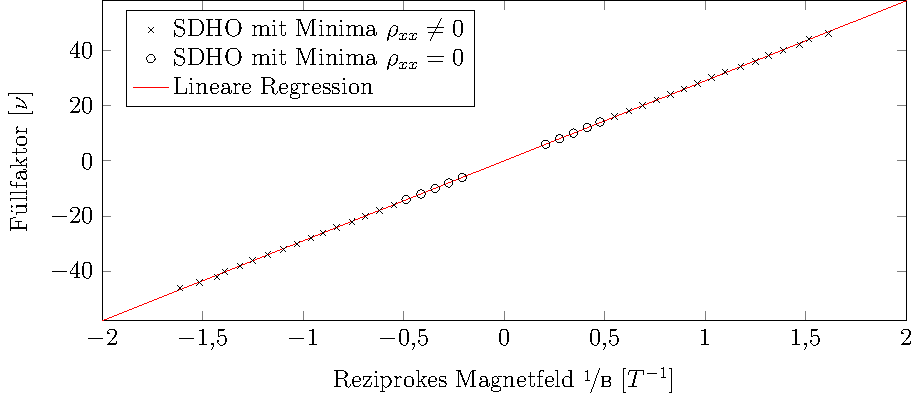
\includegraphics{graphs/ac/auswertung.pdf}
	\caption[Auswertung Füllfaktor Wechselstrommessung]{
		Auswertung Füllfaktor Wechselstrommessung.
	}
	\label{fig:ac_sdho_ausw}
\end{figure}

\begin{equation}
\nu= A\cdot \nicefrac{1}{B}=(28.908\pm 0.035)T \cdot \nicefrac{1}{B}
\end{equation}

Es wurde ein Offset von $\nu=5$ benutzt.